\documentclass{beamer}

\usepackage[utf8]{inputenc}
\usepackage[T1]{fontenc}
\usepackage[english]{babel}
\usepackage{hyperref}
\usetheme{Madrid}

%time (sec) dans graphe
%aggrandir dans le parallel nb execution

\makeatletter
\setbeamertemplate{footline}{
  \leavevmode%
  \hbox{%
  \begin{beamercolorbox}[wd=.2\paperwidth,ht=2.25ex,dp=1ex,center]{author in head/foot}%
    \usebeamerfont{author in head/foot}\insertshortauthor
  \end{beamercolorbox}%
  \begin{beamercolorbox}[wd=.55\paperwidth,ht=2.25ex,dp=1ex,center]{title in head/foot}%
    \usebeamerfont{title in head/foot}Presentation INRIA
  \end{beamercolorbox}%
  \begin{beamercolorbox}[wd=.25\paperwidth,ht=2.25ex,dp=1ex,right]{date in head/foot}%
    \usebeamerfont{date in head/foot}\insertshortdate{}\hspace*{2em}
    \insertframenumber{} / \inserttotalframenumber\hspace*{2ex} 
  \end{beamercolorbox}}%
  \vskip0pt%
}
\makeatother
\title{Code performance analysis and improvement by optimizing compilation : Case study}

%\subtitle{Master 1 Computer Science}

\author[Pierre \textsc{Tassel}]{Pierre \textsc{Tassel} under the supervision of Pr. \textsc{Touati}}

\institute[Universitée Nice Sophia Antipolis] 
{Département of Computer Science\\
University of Nice Sophia-Antipolis
\and
Student in Master of Computer Science}

\date{\today}

\subject{Présentation TER}

% Let's get started
\begin{document}
%\author{Pierre \textsc{Tassel}}
\begin{frame}
  \titlepage
\end{frame}

\begin{frame}{Outline}
  \tableofcontents
  % You might wish to add the option [pausesections]
\end{frame}

% Section and subsections will appear in the presentation overview
% and table of contents.
\section{The program}

\begin{frame}{The program}{MinMax for the Awale game}
\begin{itemize}
    \item 
    AI for Awale's game with 6 row and 4 seed per row.
  \item
    Writen in C++ by Pr \textsc{Régin}.
  \end{itemize}
  \begin{figure}
   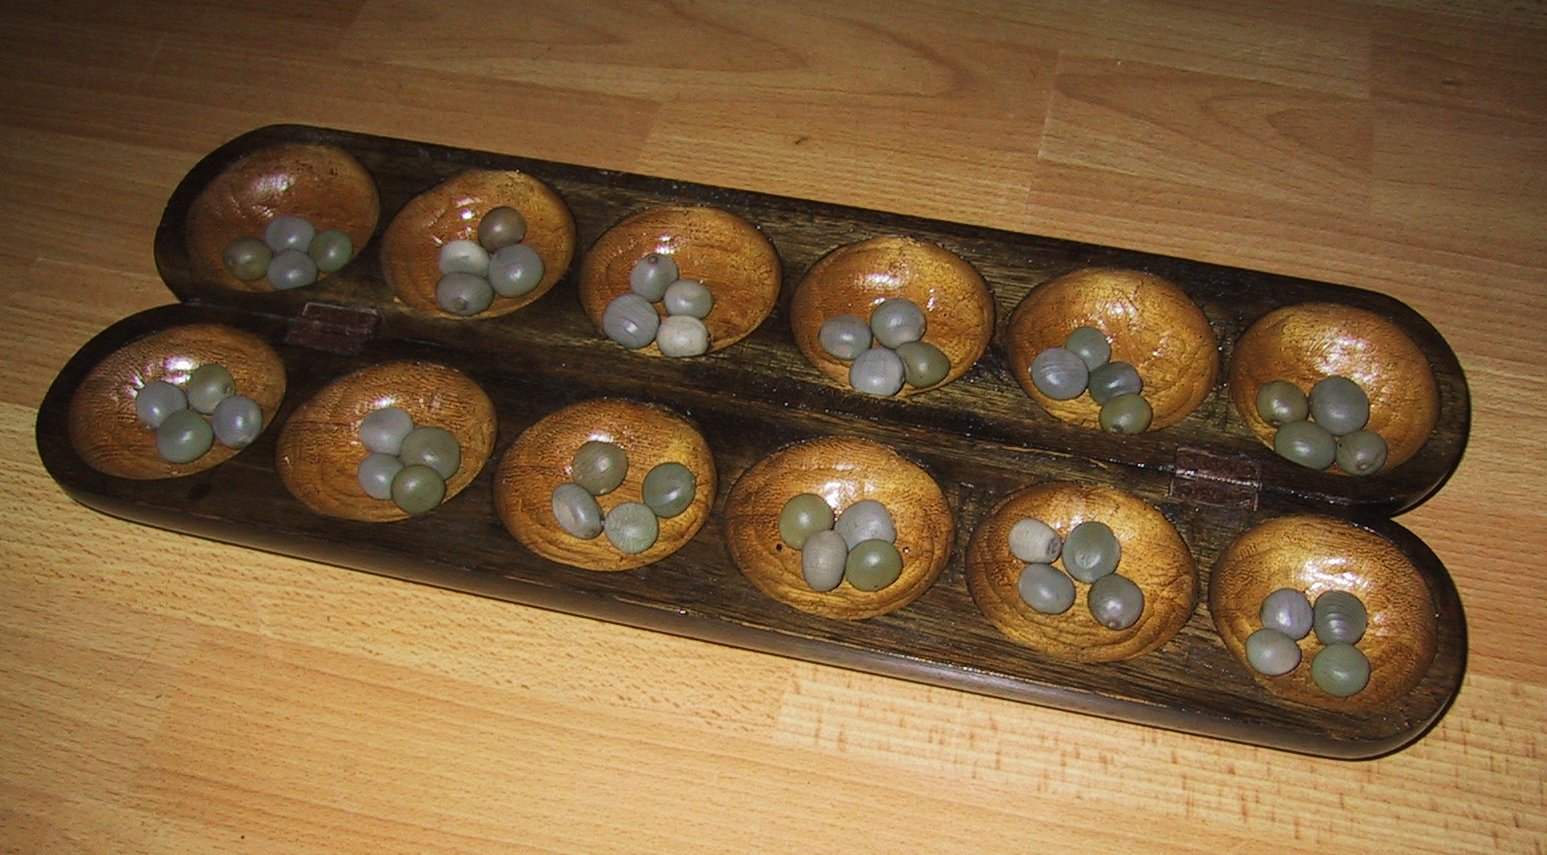
\includegraphics[width= 0.7\linewidth, keepaspectratio]{Awale.jpg}
   \caption{The Awale's game.\label{Fig:awale}}
\end{figure}
\end{frame}

\begin{frame}{The program}{MinMax with Alpha Beta prunning}
  \begin{figure}
   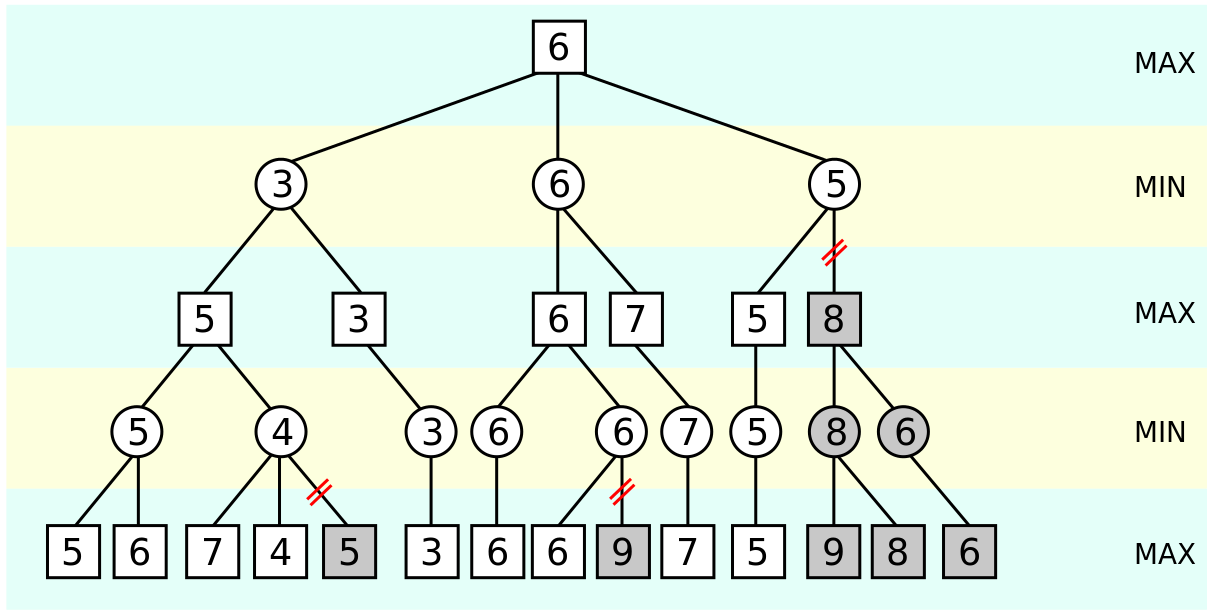
\includegraphics[width= 0.9\linewidth, keepaspectratio]{AB_pruning.png}
\end{figure}
\end{frame}

\section{Experimental approach}
\begin{frame}{Experimental approach}{Hardware and software environment}
\begin{itemize}
  \item
  	\textit{Processeur Scaling} desactivated, Intel Xeon 4 core 2,66GHz processor, 4Go DDR3, 512GB of HDD.
  \item
    Minimalist CLI environement, Arch Linux based on Linux 4.14.13-1.
    \item
    Three compiler analysed\,: GCC, ICC and CLang (all up to date).
    \item
    Input file generated by playing the program against itself, deterministic program.
    \item
    The executions are repeated 20 times for each tested configuration.
\end{itemize}
\end{frame}

\section{Analysis and optimization of sequential performances}

\begin{frame}{Analysis and optimization of sequential performances}

\begin{figure}
      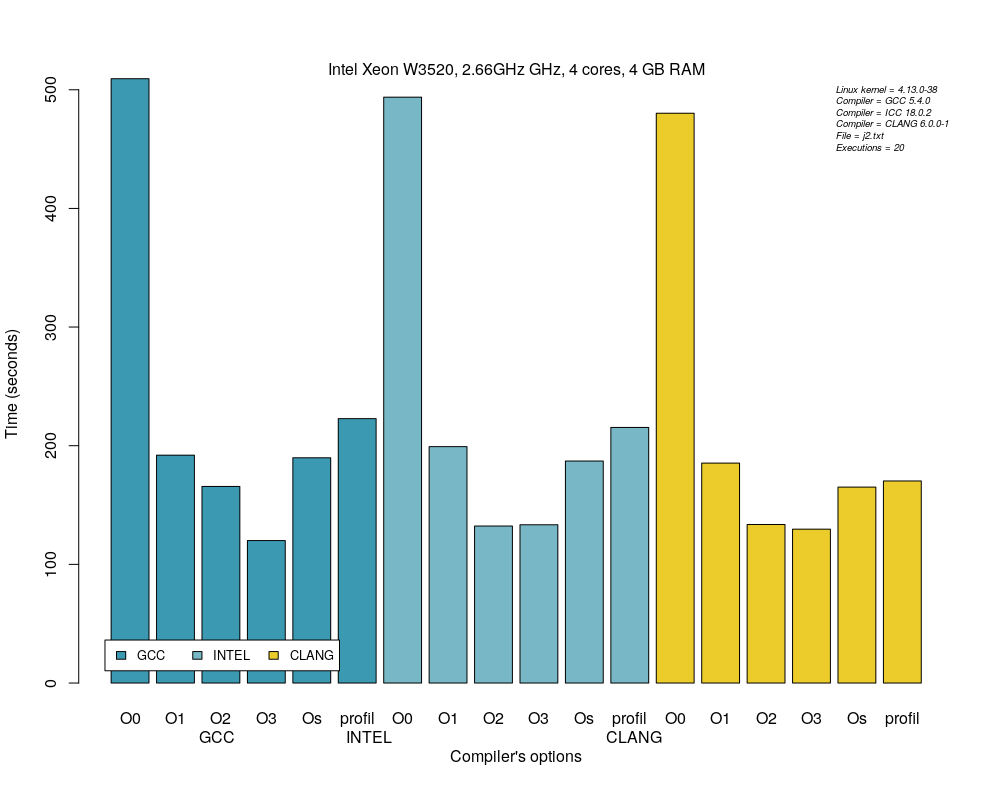
\includegraphics[width=0.7\textwidth]{GCCvsICCvsCLANG_j2.png}
      \caption{Sequential execution time when the program starts.}
\end{figure}
\end{frame}

\begin{frame}{Code performance profiling}{GProf}
\begin{figure}
        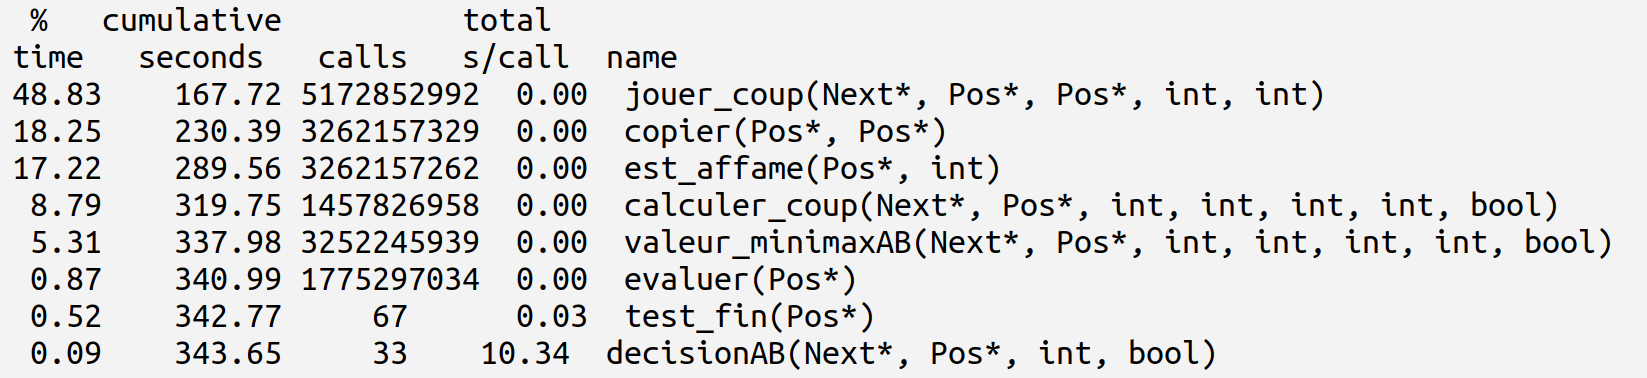
\includegraphics[width=\textwidth]{gprof.png}
        \caption{Code Profiling with GProf.\label{Fig:GProf}}
\end{figure}
\end{frame}

\begin{frame}{Code performance profiling}{vTune}
\begin{columns}
    \column{6.5cm}
    \begin{figure}
      \centering
   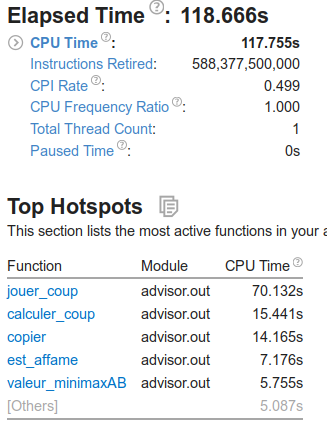
\includegraphics[width=0.75\textwidth]{vtune.png}
   \caption{vTune processor usage analysis.\label{Fig:vTune_proc}}
    \end{figure}
    \column{6.5cm}
    \begin{figure}
      \centering
   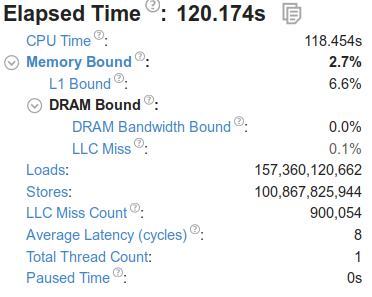
\includegraphics[width=0.9\textwidth]{memory_vtune.png}
   \caption{vTune memory usage analysis.\label{Fig:vTune_mem}}
    \end{figure}
    
  \end{columns}
\end{frame}

\section{Adding parallelism}

\begin{frame}{Naïve approach to adding parallelism}
	\begin{figure}
      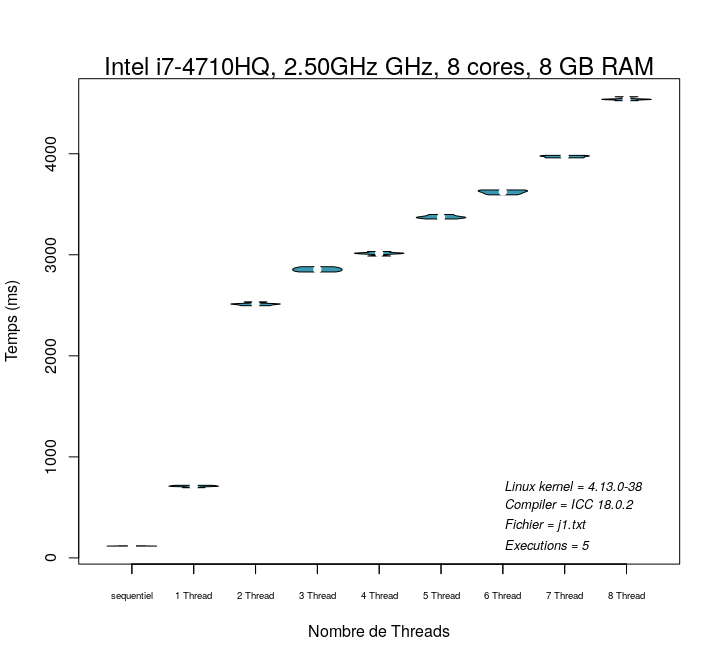
\includegraphics[width=0.7\textwidth]{intel_parallel_naif.png}
      \caption{Result of added parallelism with Intel compiler.\label{Fig:naif_intel}}
  
	\end{figure}
\end{frame}

\begin{frame}{False Sharing}
	\begin{figure}
	\begin{columns}
      \column{.72\linewidth}
      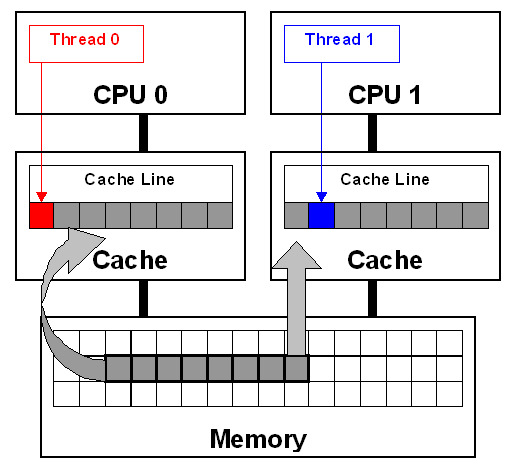
\includegraphics[width=\textwidth]{false_sharing.jpg}
      \column{.25\linewidth}
      \caption{False Sharing.\label{Fig:false_sharing}}{\href{https://software.intel.com/en-us/articles/avoiding-and-identifying-false-sharing-among-threads}{Source : Intel's Documentation.}}
    \end{columns}	
    \end{figure}
\end{frame}

\begin{frame}{Thread Affinity}
	\begin{figure}
	\begin{columns}
      \column{.25\linewidth}
      \caption{Analyzing the impact of thread placement with the Intel compiler, \textbf{-O3} with 8 CPUs.\label{Fig:thread_affinity}}
      \column{.72\linewidth}
      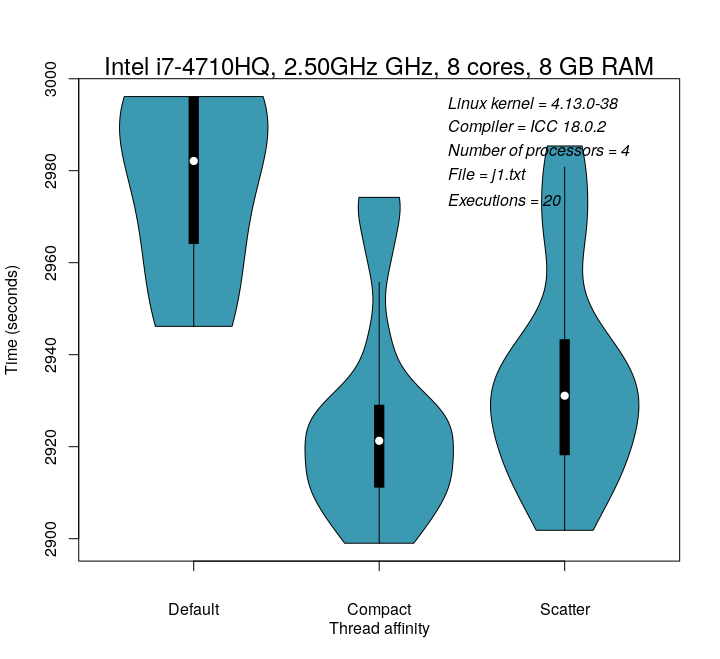
\includegraphics[width=\textwidth]{defaultVSscatterVScompact.png}
    \end{columns}	
	\end{figure}
\end{frame}

\begin{frame}{Intel Advisor}
	\begin{figure}
	\begin{columns}
      \column{.60\linewidth}
      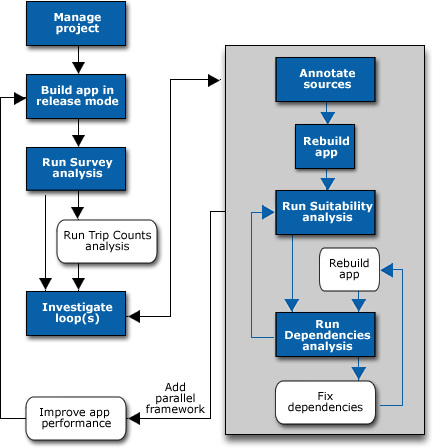
\includegraphics[width=\textwidth]{Intel.jpg}
      \column{.25\linewidth}
      \caption{Iterative method to add parallelism (proposed by Intel).\label{Fig:intel_iter}}{\href{https://software.intel.com/en-us/articles/avoiding-and-identifying-false-sharing-among-threads}{Source : Intel's Documentation.}}
    \end{columns}	
    \end{figure}
\end{frame}


\begin{frame}{Difficulties of code optimization}
\begin{itemize}
\item
Very sequential algorithm.
\item
Low number of iterations ($n = 6$).
\item
Lot of usage of pointers that could blind the compiler's optimisation passes.
\end{itemize}
\end{frame}

\section{Simple algorithmic modification}


\begin{frame}{Simple algorithmic modification}

\begin{itemize}
  \item
  Sort the "moves" to evaluate.
  \item
  Transposition table.
  \item
  Padding to remove False Sharing.
  \item
  Modify algorithm to add parallelism.
 \end{itemize}	
\end{frame}

\begin{frame}{Sort the "moves"}
	\begin{figure}
      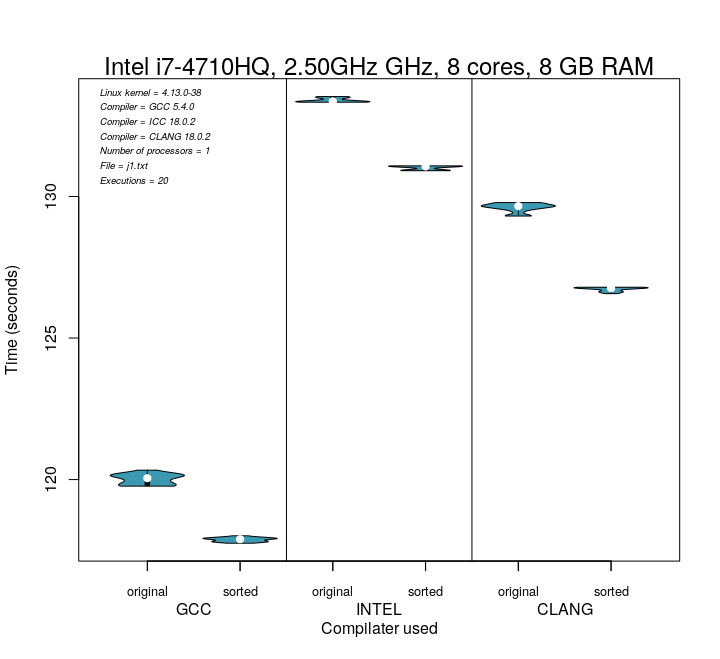
\includegraphics[width=0.7\textwidth]{trie.png}
      \caption{Analysis of the impact of the sorted move.\label{Fig:trie}}
	\end{figure}
\end{frame}

\begin{frame}{Transposition table}
	\begin{figure}
	\begin{columns}
      \column{.5\linewidth}
      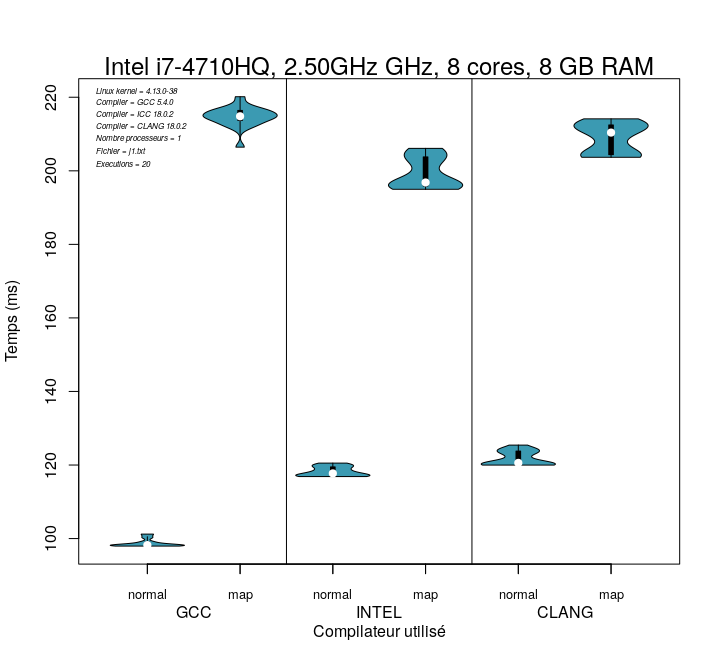
\includegraphics[width=\textwidth]{sorted_map.png}
      \caption{Binary search tree.\label{Fig:arbre_binaire}}
      \column{.5\linewidth}
      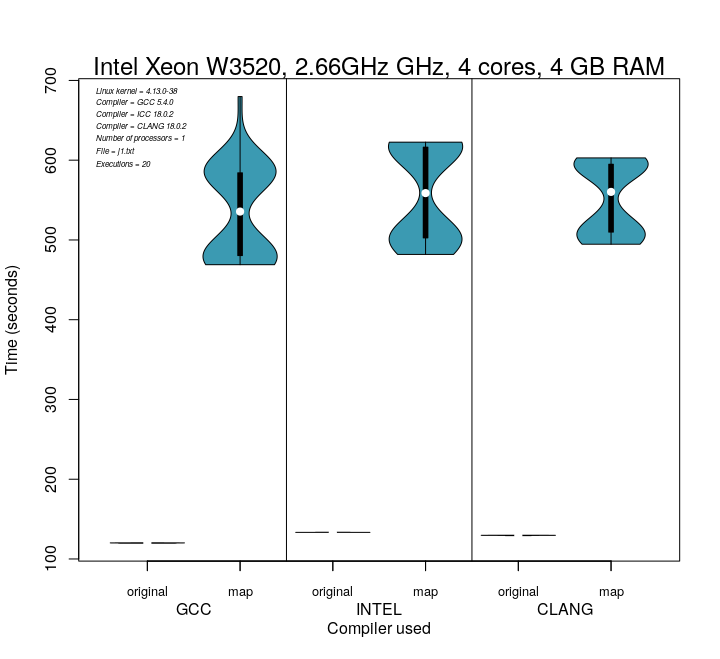
\includegraphics[width=\textwidth]{unsorted_map.png}
      \caption{Hash table.\label{Fig:arbre_binaire}}
    \end{columns}	
	\end{figure}
\end{frame}

\begin{frame}{Padding}
	\begin{figure}
      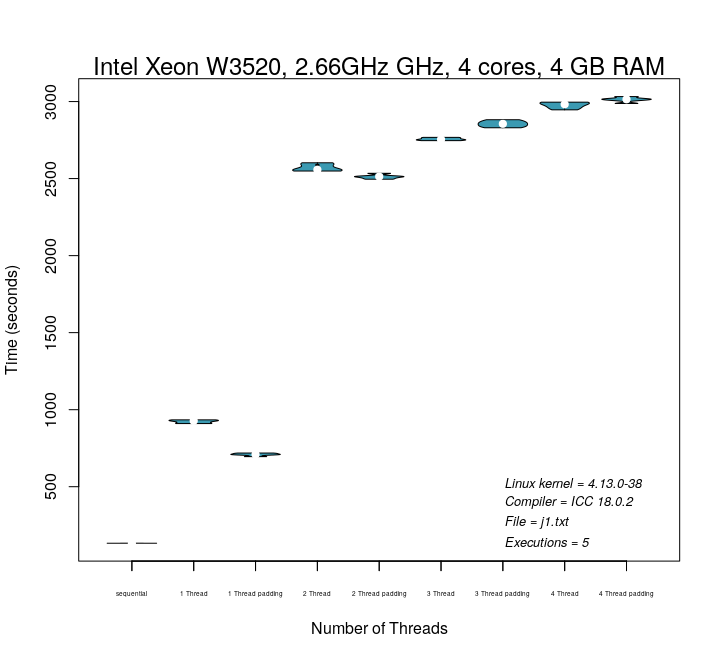
\includegraphics[width=0.7\textwidth]{padding.png}
      \caption{Padding to remove False Sharing.\label{Fig:trie}}
	\end{figure}
\end{frame}

\begin{frame}{New parallel version}
	\begin{figure}
      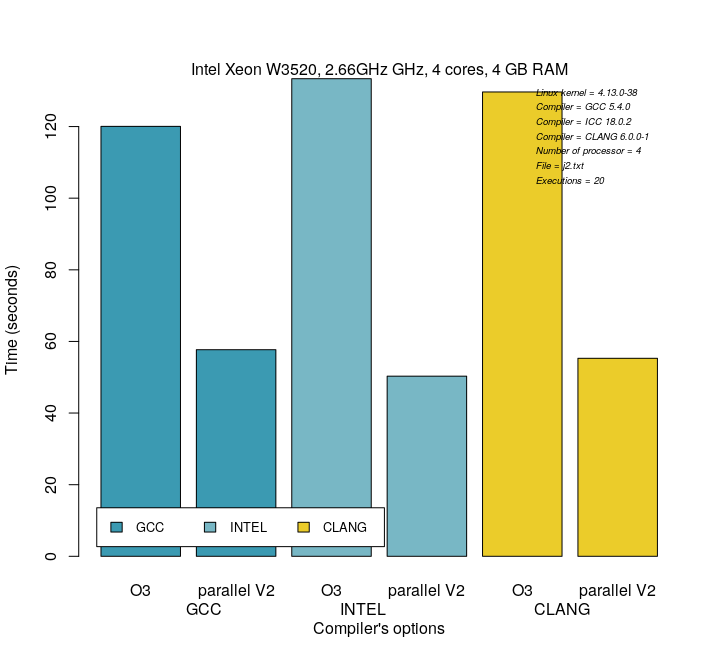
\includegraphics[width=0.7\textwidth]{parallel_v2.png}
      \caption{New parallel version.\label{Fig:trie}}
	\end{figure}
\end{frame}

\section{Conclusion}

\begin{frame}{Conclusion}
\begin{itemize}
	\item
	GCC beats ICC for a sequential code on Intel's architecture.
	%spectre benchmark
	\item
	Parallelization with OpenMP can severely degrade performance.
  \item
    False Sharing phenomena.
  \item
  	Algorithmic changes needed to improve performance.
 \end{itemize}	
\end{frame}

\section{Perspectives}

\begin{frame}{Perspectives}
\begin{itemize}
	\item
	Thread affinity on the new version.
 \end{itemize}	
\end{frame}

\end{document}


